% !Mode:: "TeX:UTF-8"
% !TEX program  = xelatex
\documentclass[a4paper]{article}
\usepackage{amsmath}
\usepackage{amssymb}
\usepackage{ctex}
\usepackage{graphicx}
\usepackage[european]{circuitikz}
\usepackage{multirow}
\usepackage{enumitem}
\usepackage{geometry}
\usepackage{hyperref}
\geometry{a4paper, top=2cm, bottom=2cm, left=2cm, right=2cm}

\begin{document}
	\section*{\Huge 编程作业四报告}
	\section*{\small 王凯灵 521030910356 2023年4月11日}
	本次作业使用的音频为未混音的半成品合成歌曲，单声道44100kHz采样导出。为防止批改时体积较大，已将原文件切割并压缩码率至较小体积。
	\section*{代码实现}
	本次作业并没有涉及原理推导。只描述代码实现过程。
	\begin{enumerate}
		\item 依据定义画图，使用了stft画图函数，对比了使用spectrogram函数作图，stft预设完整，使用方便，结果清晰。结果图如图1所示。
		\item 使用了resample函数进行下采样，由于44100k下采样时不能一一映射，代码中另外手动实现了取整方法的下采样，即对于应重采样的间隔数取整。对比两者效果无肉眼可分辨区别。另有插值重采样的方法，经过阅读源码，确定resample函数默认使用插值重采样，但可选使用取整方法。下采样结果如图2，3，4所示。可以发现，频谱时间分辨率降低，但频率分辨率提高。对应的音频文件为audio\_*kHz.wav。
		\item 使用了interp1函数进行一维插值，结果如图5，6，7所示，由于精度问题，插值的时间和原信号时间有微量偏移。为了合理的量化与原信号的误差，使用五点均差衡量重建信号与原信号的残差audio\_*kHz\_interp.wav。
		\item 使用butter函数实现了十个二阶带通滤波器。其中，这十个频率从30Hz开始，依据梅尔频率公式，$f_m = 2595 \log_{10}(1+\frac{f}{700})$，各个滤波器的中心频率依据非线性刻度，使用指数级上升至15360Hz。根据理论计算，设计的带通滤波器两两之间有10\%重叠，最小频率覆盖到约26.8367，最大频率覆盖到约16979.5714，尽可能覆盖了人耳全频率。
		
		图8显示了我的均衡器的一次均衡结果，使用的增益为$[-3~-1~1~1~2~3~2~1~1~1]$，希望增强华华的声音。
		
		实际上，我把我的均衡器封装为了一个app，但使用了htmlUI，并没有使用MATLAB APPdesigner，因为这个工具竟然只支持.mlapp格式到.m的单向转换，而不支持转回，意味着如果希望自由编辑代码，就无法使用可是化APP设计工具，相比于Qt可以说极其落后。于是我是用纯代码实现，支持自由调整滑动条更改均衡器和键入，支持自由选择和保存文件，支持时域自适应绘图，支持应用内播放。我将代码发布为了mlapp安装包，在我的多个设备上均可以使用。	
	\end{enumerate}

	\newpage
	\section*{附录}
	\begin{figure}[h!]
		\centering
		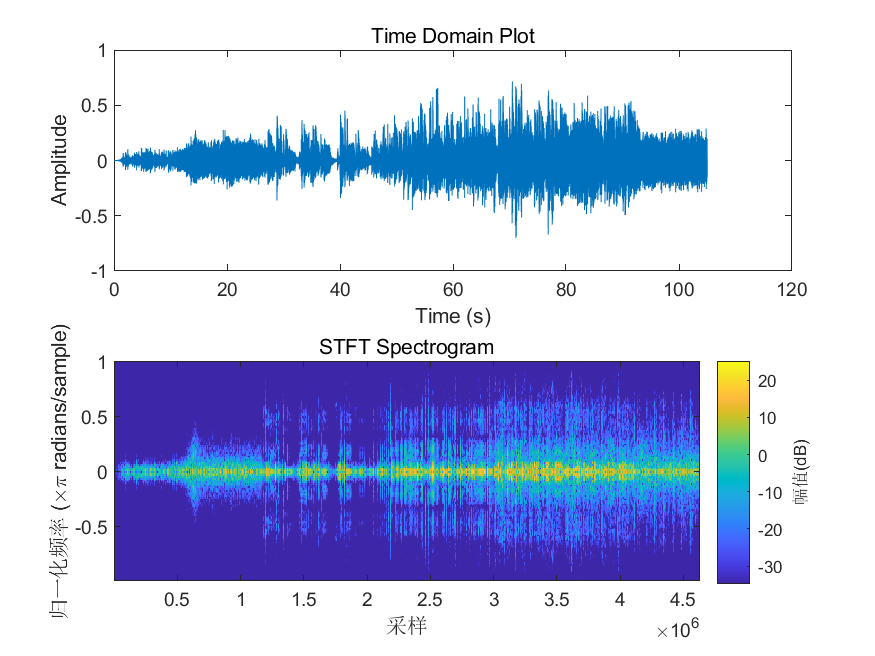
\includegraphics[width=0.75\textwidth]{../figures/stftp}
		\caption{原音频时域图和STFT图}
	\end{figure}
	\begin{figure}[h!]
		\centering
		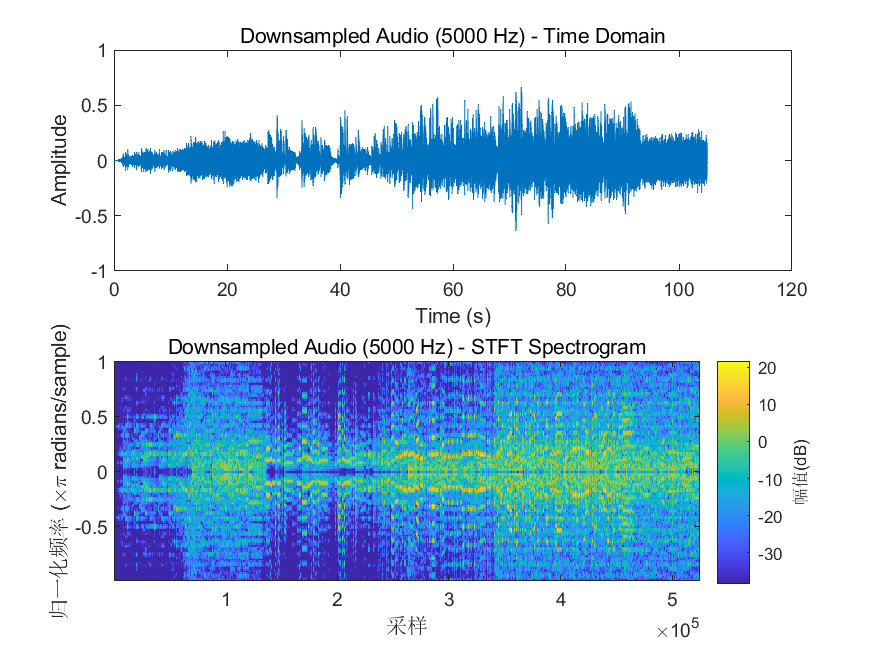
\includegraphics[width=0.75\textwidth]{../figures/ds5000}
		\caption{下采样5000kHz时域图和STFT图}
	\end{figure}
	\begin{figure}[h!]
		\centering
		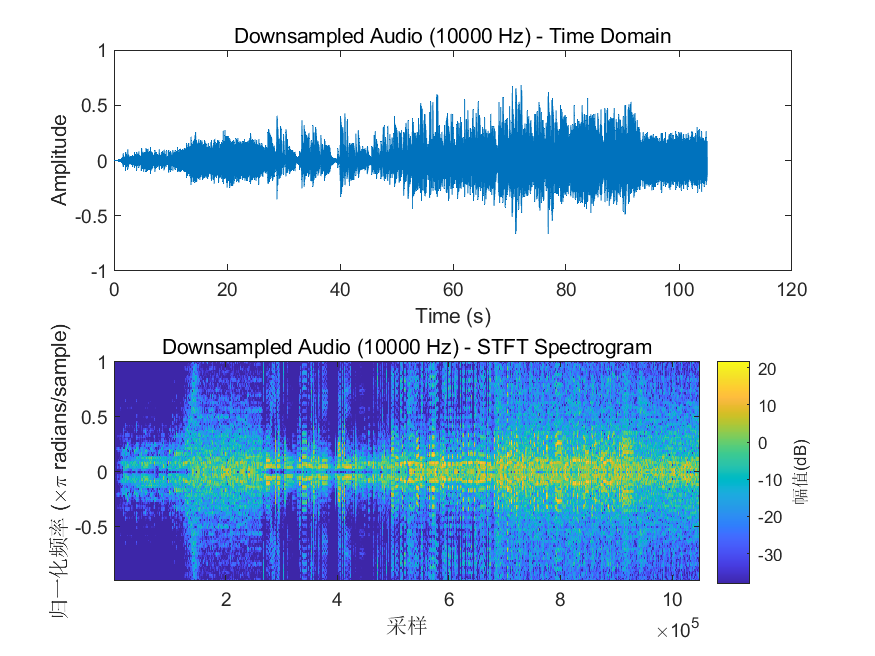
\includegraphics[width=0.75\textwidth]{../figures/ds10000}
		\caption{下采样10000kHz时域图和STFT图}
	\end{figure}
	\begin{figure}[h!]
		\centering
		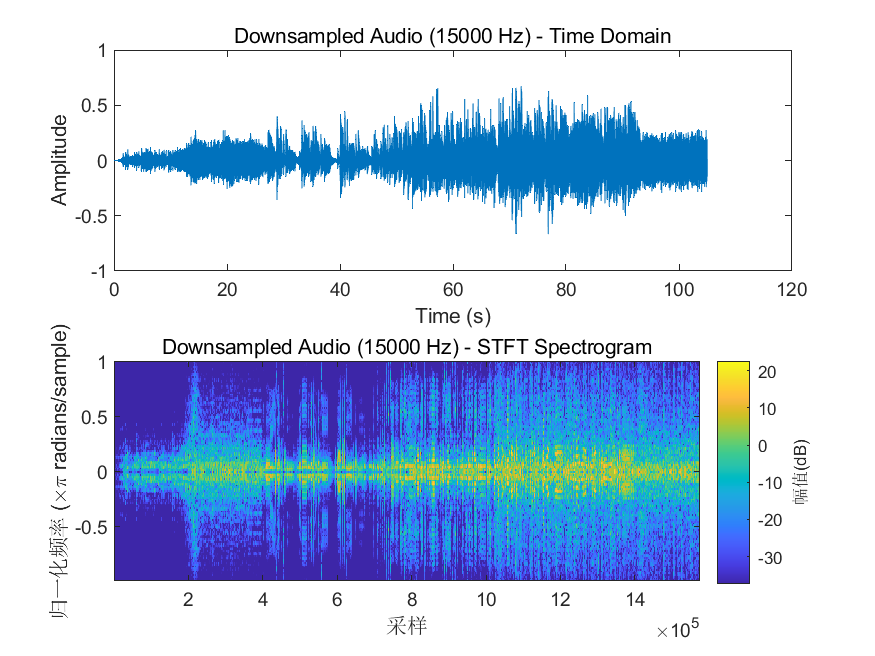
\includegraphics[width=0.75\textwidth]{../figures/ds15000}
		\caption{下采样15000kHz时域图和STFT图}
	\end{figure}
	\begin{figure}[h!]
		\centering
		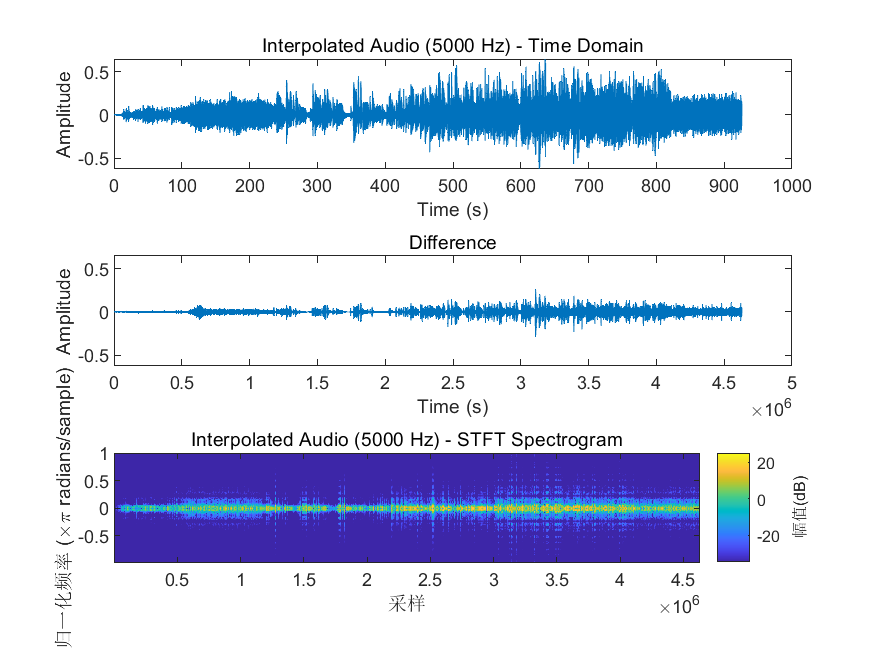
\includegraphics[width=0.75\textwidth]{../figures/in5000}
		\caption{插值5000kHz时域图，残差和STFT图}
	\end{figure}
	\begin{figure}[h!]
		\centering
		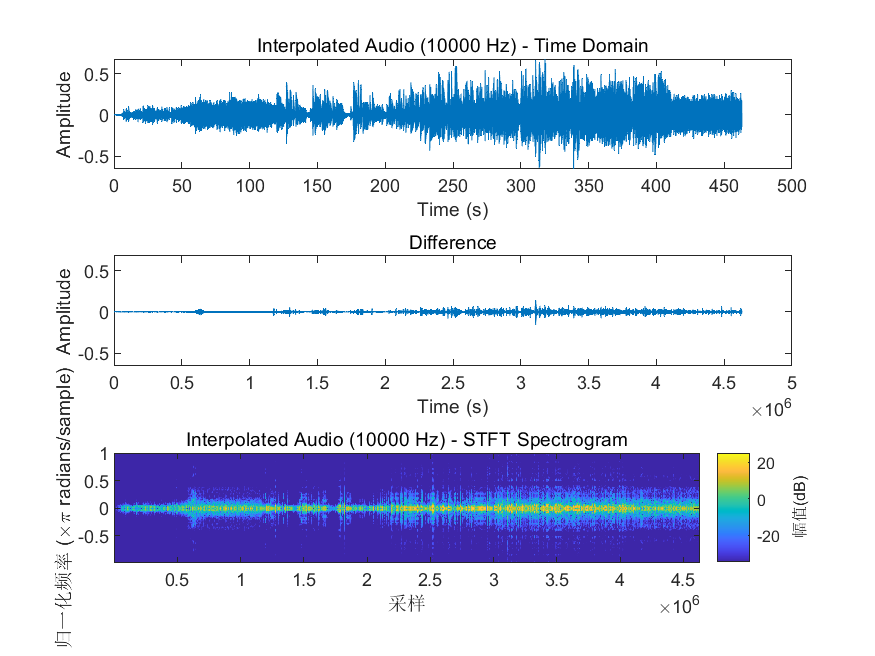
\includegraphics[width=0.75\textwidth]{../figures/in10000}
		\caption{插值10000kHz时域图，残差和STFT图}
	\end{figure}
	\begin{figure}[h!]
		\centering
		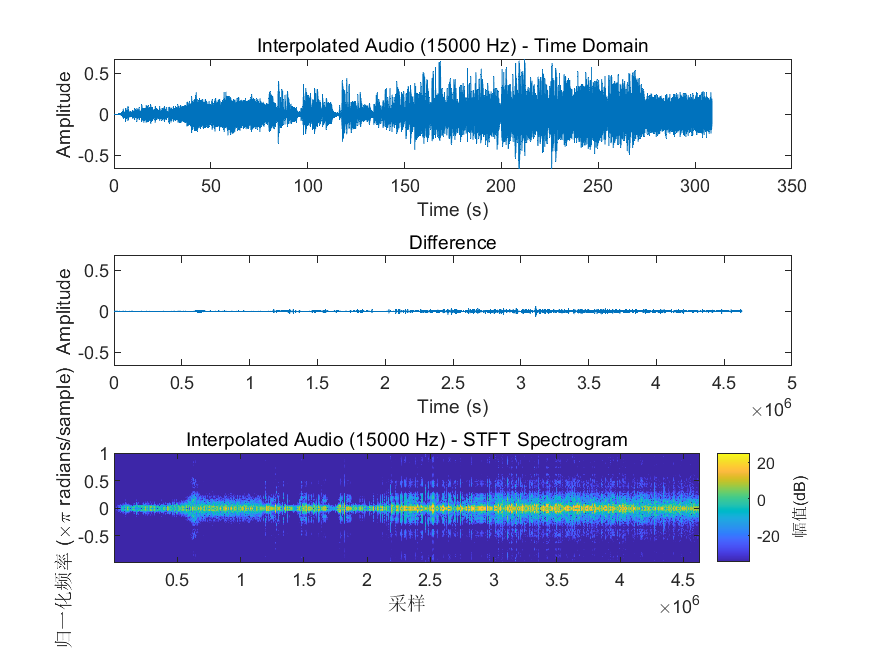
\includegraphics[width=0.75\textwidth]{../figures/in15000}
		\caption{插值15000kHz时域图，残差和STFT图}
	\end{figure}
	\begin{figure}[h!]
		\centering
		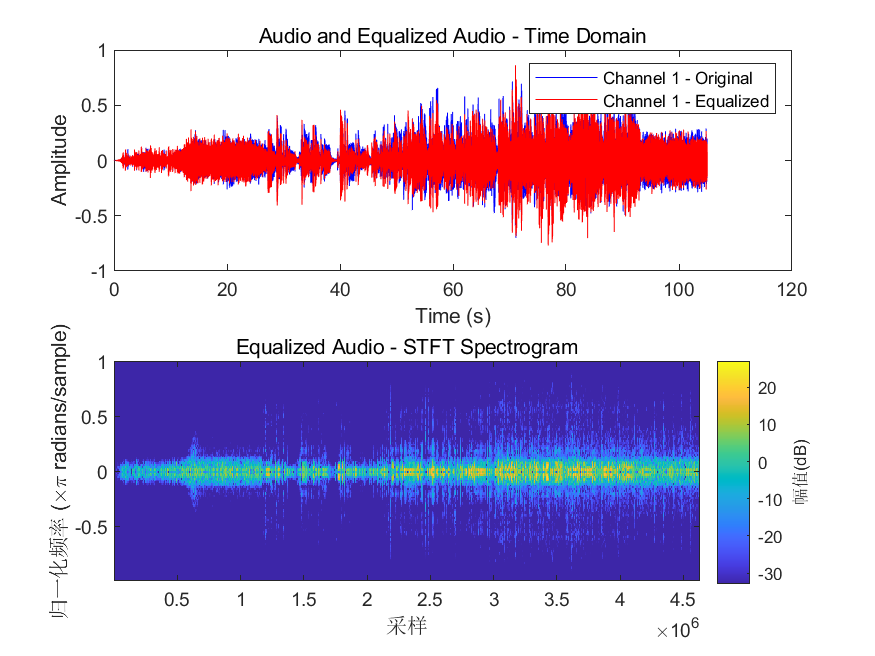
\includegraphics[width=0.75\textwidth]{../figures/audio_eq_stft}
		\caption{均衡器增强华华结果}
	\end{figure}
\end{document}